\chapter{Arcade Machine Setup}
\label{cha:arcade_machine_setup}

This chapter explains how to assemble the arcade machine hardware and install the software needed to run RetroPie on the Raspberry Pi.  

\section{Hardware Assembly}
\label{sec:hardware_assembly}

The hardware assembly stage involves preparing and connecting all physical components of the arcade machine. This includes mounting the joysticks and buttons, wiring them to the USB encoder, and linking the encoder and other peripherals to the Raspberry Pi.


\subsection{Installing Joysticks and Buttons}
\label{subsec:installing_joysticks_buttons}
Mount the joysticks and buttons onto the arcade panel, securing them firmly with screws or mounting plates. Ensure that the buttons are arranged in a comfortable layout for gameplay. While the layout can be adjusted to personal preference, this project follows the configuration shown below.
\\
\begin{figure}[htb] 
	\centering  
	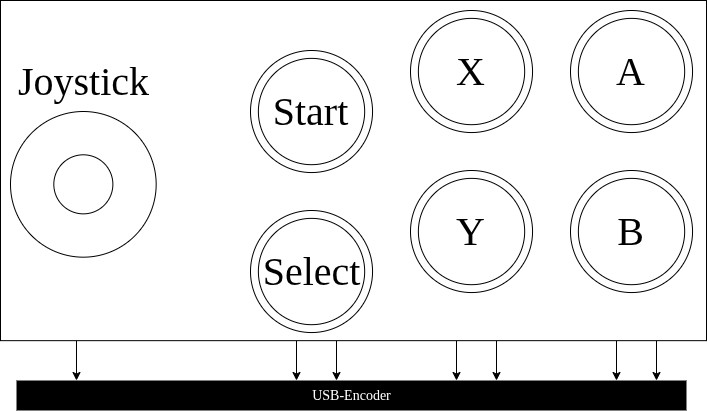
\includegraphics[scale=0.35]{F_Figures/button_layout.png}
	\caption{Joystick and button layout.}
	\label{fig:button_layout}
\end{figure} 

\subsection{Connecting USB Encoder}
\label{subsec:connecting_usb_encoder}
Attach the button and joystick wires to the USB encoder according to Figure 4.2. The encoder converts physical inputs into signals recognized by the Raspberry Pi over USB.
 Note that the joystick uses 5-pin, arcade buttons use 3-pin cable for connection. 
\\
\begin{figure}[htb] 
	\centering  
	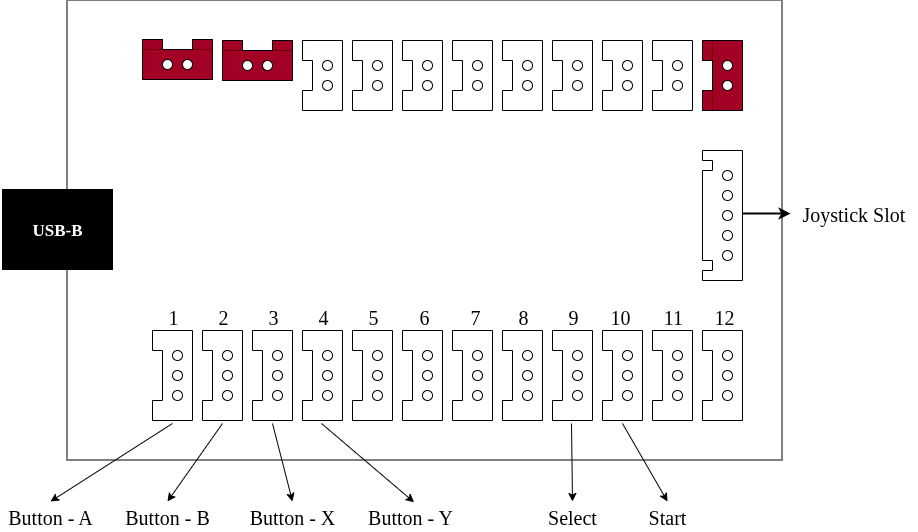
\includegraphics[scale=0.26]{F_Figures/usb_encoder_layout.png}
	\caption{USB-encoder wiring schema.}
	\label{fig:usb_encoder_layout}
\end{figure} 

\subsection{Wiring to Raspberry Pi}
\label{subsec:wiring_raspberry_pi}
In order to complete the setup, all connections must be completed before running Raspberry Pi. Connect the USB encoder to the Raspberry Pi using a standard USB cable. Also connect a keyboard to Raspberry Pi using USB port. 
A display must be connected to HDMI port. Connecting a speaker is optinal. These steps provides all the necessary connections to complete the hardware assembly, except power supply. Once micro-USB power is inserted to the Raspberry, the system will start up. 
Figure 4.3 shows the fully-connected system schema. 
\\
\begin{figure}[htb] 
	\centering  
	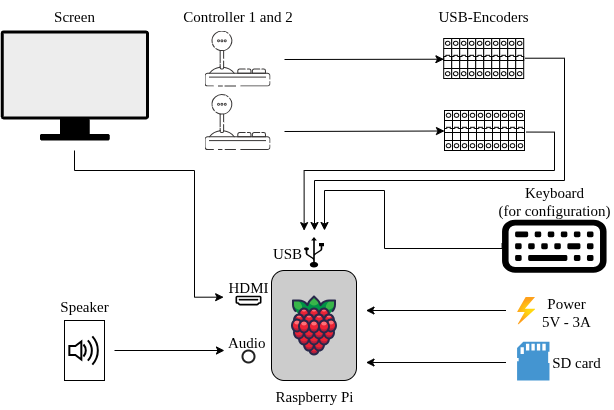
\includegraphics[scale=0.285]{F_Figures/system_schema.png}
	\caption{Fully-connected system schema.}
	\label{fig:system_schmema}
\end{figure} 

\section{Software Installation}
\label{sec:software_installation}
Raspberry Pi doesn't have any storage unit than the SD card. It requires a SD card with a system image to boot up. 
In this project, RetroPie image in the SD card runs on the Raspberry Pi.
\subsection{Booting from SD Card}
\label{subsec:booting_sd_card}
Insert the prepared SD card with the RetroPie image into the Raspberry Pi and power it on. On first boot, the system will expand the filesystem and load into the RetroPie setup screen, where initial configuration and controller mapping can be completed.  
